\chapter{\ifenglish Background Knowledge and Theory\else ทฤษฎีที่เกี่ยวข้อง\fi}

การทำโครงงาน เริ่มต้นด้วยการศึกษาค้นคว้า ทฤษฎีที่เกี่ยวข้อง หรือ งานวิจัย/โครงงาน ที่เคยมีผู้นำเสนอไว้แล้ว ซึ่งเนื้อหาในบทนี้ก็จะเกี่ยวกับการอธิบายถึงสิ่งที่เกี่ยวข้องกับโครงงาน เพื่อให้ผู้อ่านเข้าใจเนื้อหาในบทถัดๆ ไปได้ง่ายขึ้น


\section{UX Design}
UX Design(User Experience Design) คือ การออกแบบเพื่อให้ผู้ใช้งานมีประสบการณ์ในการใช้งานที่ดีในเว็ปไซต์ หรือแอพพลิเคชันนั้นๆ
ไม่ว่าจะเป็นความง่ายในการใช้งาน ความต่อเนื่องในการใช้งาน การสื่อความหมาย ฯลฯ ตาม UX Law\cite{uxlaw} เพื่อประสบการณ์การที่ดีที่สุดของผู้ใช้งาน

\section{เครื่องมือที่ใช้ในการพัฒนา}
\subsection{React}
React เป็น Framework ที่ใช้งานกับ JavaScript ในการสร้างหน้า Fontend โดย React นั้นสามารถจัดการกับความซับซ้อนของระบบการทำงานได้โดยจะแบ่งส่วนการทำงานต่างๆออกจากกัน
เป็นส่วนเล็กๆที่สามารถจัดการได้ง่าย เช่น ส่วนของการแสดงผล ส่วนของงการทำงาน และในส่วนของการจัดการตัวแปร และในแต่ละส่วนก็จะแยกออกเป็นแต่ละระบบ เช่น ระบบล็อกอิน ระบบแดชบอร์ด ระบบจัดการสร้างทัวร์นาเมนต์ ฯลฯ 
ทำให้การจัดการนั้นง่าย และมีประสิทธิภาพ เนื่องจากเราสามารถรู้ได้ว่าจุดไหนมีปัญหาในการการทำงาน โค้ดสามารถอ่านได้ง่ายไม่เยอะจนเกินไป หลังจากนั้นค่อยนำมารวมกันโดยเรียกใช้ส่วนนั้นๆ และ React ยังมีตัวช่วยในการจัดการกับ State การทำงานของระบบ และจัดการกับ DOM
เมื่อมีการเปลี่ยนแปลงของข้อมูลใน DOM ได้ทันที และมากไปกว่านั้น React ได้ถูกใช้งานมาเป็นเวลานานทำให้มี UI Library ให้ใช้งานในการแสดงผลหน้าเว็ป และยังมีแหล่งข้อมูลในการหาความรู้ในการพัฒนาระบบเป็นจำนวนมากทำให้ง่าย และร่วดเร็วในการพัฒนาแพรตฟอร์มขึ้นเป็นอย่างมาก 

\begin{figure}[h]
    \begin{center}
    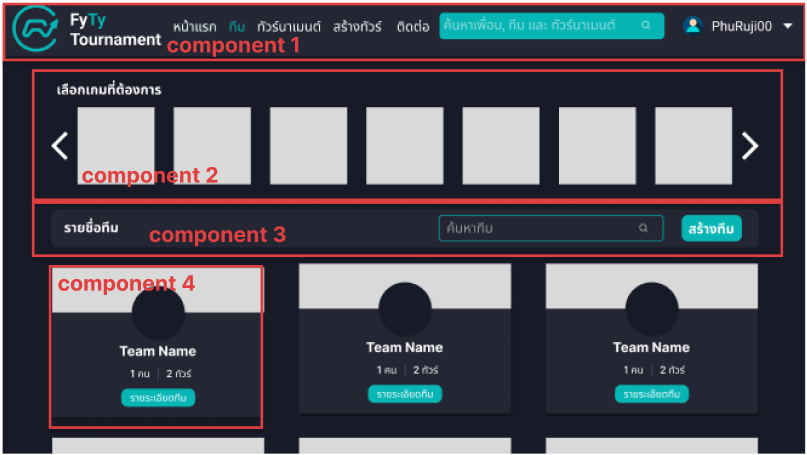
\includegraphics[width=10cm,height=10cm,keepaspectratio]{component.png}
    \end{center}
    \caption[การแยกส่วนต่างๆเป็น Component]{การแยกส่วนต่างๆเป็น Component}
    \label{fig:การแยกส่วนต่างๆเป็น Component}
\end{figure}

\begin{figure}[h]
    \begin{center}
    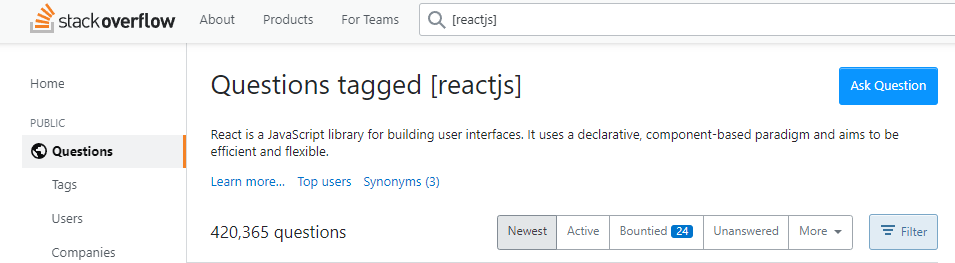
\includegraphics[width=10cm,height=10cm,keepaspectratio]{stack overflow.png}
    \end{center}
    \caption[คำถามใน Stack overflow]{คำถามใน Stack overflow}
    \label{fig:คำถามใน Stack overflow (ค้นหาเมื่อ 14/10/2565)}
\end{figure}

\subsection{Nest และ TypeScript}
Nest เป็น Framework ของ Node.js ในการจัดการ Appliction ฝั่ง Backend โดย Nest จะใช้งานร่วมกับ TypeScript 
โดย Nest นั้นสามารถขยายได้ง่าย มีการทำงานเป็นระบบแยกเป็นส่วนๆได้ ทำให้ง่ายต่อการจัดการ และการใช้ภาษา TypeScript นั้นทำให้เขียนโค้ดได้
functional มีการกำหนดชนิดของตัวแปรชัดเจนทำให้การจัดการกับข้อมูลที่เข้ามาและส่งไปได้ถูกต้อง และหาบัคนั้นได้ง่าย

\subsection{PostgreSQL และ Firebase Cloud Storage}
PostgreSQL นั้นมีการจัดการ และจัดเก็บข้อมูลในรูปแบบ structure ซึ่งเหมาะในการจัดการระบบที่ต้องการความแม่นยำ และถูกต้อง
แต่ไม่สามารถเก็บภาพ หรือวีดีโอได้ ทำให้เราต้องใช้Firebase Clound Storage เข้ามาช่วยโดยทำการอัพโหลดรูป หรือวีดีโอขึ้นไปเก็บไว้บน Firebase และรับลิ๊งของรูปภาพหรือวีดีโอ
มาเก็บไว้ใน PostgreSQL Database เพื่อในมาเรียกใช้งานภาพหลัง เนื่องจากในแพรตฟอร์มนี้จะมีการเก็บรูปภาพหลักกฐานการแข่งขันด้วยทำให้ต้องมีระบบส่วนนี้เข้ามาลองรับการใช้งาน

\begin{figure}[h]
    \begin{center}
    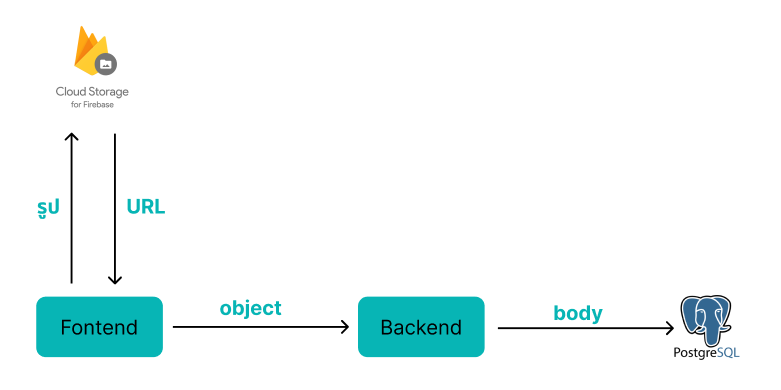
\includegraphics[width=10cm,height=10cm,keepaspectratio]{firebase.png}
    \end{center}
    \caption[การจัดเก็บรูปภาพ]{การจัดเก็บรูปภาพ}
    \label{fig:การจัดเก็บรูปภาพ}
\end{figure}

\subsection{Docker}
Docker ใช้ในการทำ Docker Images และในไปลงใน Docker Container เพื่อในไป Deploy โดยข้อดีของการใช้ Docker คือเราสามารถ  Container ที่เดียวสามารถ Deploy ได้ทุกที่ที่มี Docker รันอยู่โดยไม่ต้องกลัวว่าจะไม่สามารถรันได้
และ ง่ายกับการขยายโดยทำเป็น microservices แยกเป็นแต่ละ Docker Container ในโปรเจคนี้จะแยกออกเป็นสอง Container ได้แก่  Fontend และ Backend 

\section{\ifenglish%
\ifcpe CPE \else ISNE \fi knowledge used, applied, or integrated in this project
\else%
ความรู้ตามหลักสูตรซึ่งถูกนำมาใช้หรือบูรณาการในโครงงาน
\fi
}

\begin{enumerate}
    \item Database: การออกแบบดาต้าเบส
    \item IT Infra and Cloud Tech: การใช้ Docker ในการทำ Docker Image และ Container เพื่อในไปใช้ Deploy
\end{enumerate}

\section{\ifenglish%
Extracurricular knowledge used, applied, or integrated in this project
\else%
ความรู้นอกหลักสูตรซึ่งถูกนำมาใช้หรือบูรณาการในโครงงาน
\fi
}

\begin{enumerate}
    \item ภาษาโปรแกรมมิ่งสำหรับทำเว็ปแอพพลิเคชัน และ Framework ที่มีประสิทธิภาพในการใช้งานเพื่อเพิ่มความสะดวก และรวดเร็วในการพัฒนาเว็ปแอพพลิเคชั่น
    \item การจัดเก็บรูปภาพ และการดึงมาใช้ร่วมกับการใช้ฐานข้อมูลแบบSQL โดยการใช้ Cloud มาเป็นตัวช่วย
\end{enumerate}
